
\documentclass{article}
\usepackage{amsmath}
\usepackage{graphicx}
\usepackage{caption}
\usepackage{geometry}
\geometry{margin=1in}

\title{VAM Beam--Swirl Interaction Spectrum}
\author{Æther Dynamics Model}
\date{}

\begin{document}
\maketitle

\section*{1. Introduction}
In the Vortex Æther Model (VAM), fusion events are governed by the overlap between external beam-induced swirl modes and the natural swirl eigenfrequencies of vortex knots. This document formalizes the interaction and presents a spectral yield curve.

\section*{2. Swirl Coupling Formalism}
We define the fusion excitation yield $Y_{\mathrm{VAM}}$ as the spectral overlap:

\begin{equation}
Y_{\mathrm{VAM}} = \int_0^\infty \rho_{\mathrm{beam}}(\omega) \cdot \sigma_{\mathrm{knot}}(\omega) \, d\omega
\end{equation}

\noindent where:
\begin{itemize}
  \item $\rho_{\mathrm{beam}}(\omega)$ is the Gaussian spectral energy density of the injected beam:
  \[
  \rho_{\mathrm{beam}}(\omega) = A \exp\left(-\frac{(\omega - \omega_0)^2}{2 \Delta \omega^2} \right)
  \]
  \item $\sigma_{\mathrm{knot}}(\omega)$ is the vortex knot's absorption spectrum modeled as a sum of Lorentzians:
  \[
  \sigma_{\mathrm{knot}}(\omega) = \sum_n \frac{B_n \Gamma_n^2}{(\omega - \omega_n)^2 + \Gamma_n^2}
  \]
\end{itemize}

\section*{3. Numerical Simulation}
We model:
\begin{itemize}
  \item A beam centered at frequency $\omega_0 = \frac{C_e}{r_c}$
  \item Three vortex species with resonances near $\omega_0$
\end{itemize}

\begin{figure}[h!]
  \centering
  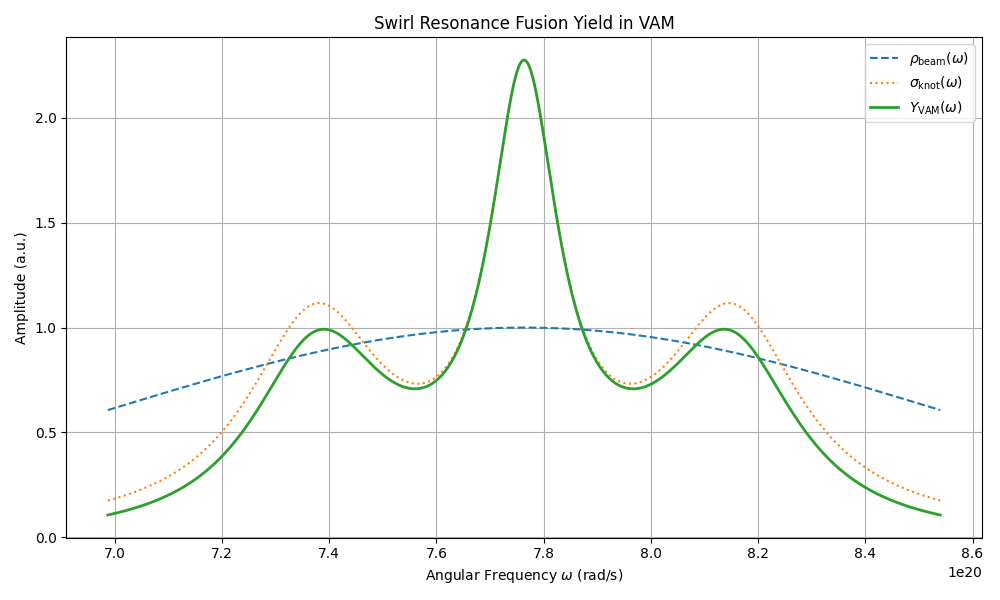
\includegraphics[width=0.9\textwidth]{images/vam_swirl_yield_plot}
  \caption{Spectral overlap of beam and vortex knot absorption functions. The fusion yield $Y_{\mathrm{VAM}}(\omega)$ peaks where resonance occurs.}
\end{figure}

\section*{4. Interpretation}
The model confirms that fusion is enhanced when the injected swirl field (from laser-accelerated ions) matches one or more knot resonance modes. Broader beams engage multiple knot species; narrow-band beams offer precision tuning for maximal yield.

\begin{figure}[h!]
  \centering
  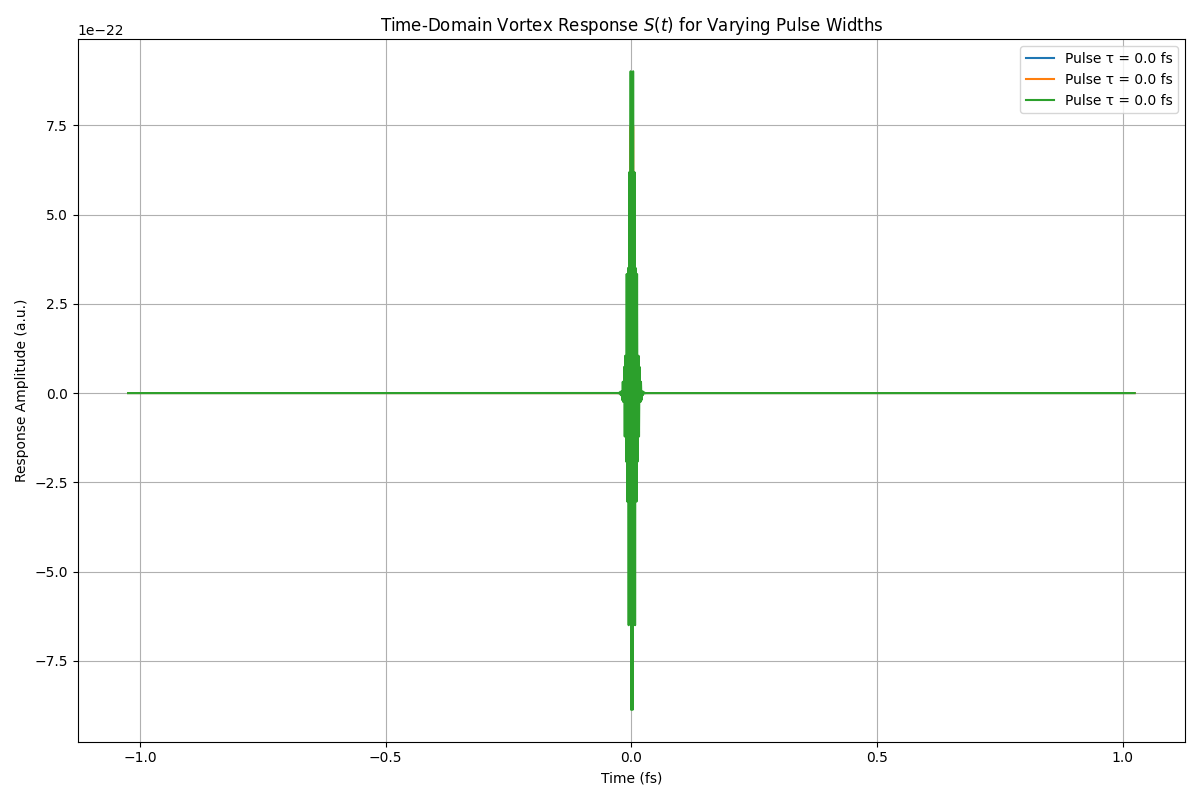
\includegraphics[width=0.9\textwidth]{images/vam_time_response_plot}
  \caption{Time-domain response $S(t)$ of the vortex knot to Gaussian pulses of various durations $\tau$. Shorter pulses excite a wider range of vortex modes, while longer pulses selectively enhance resonant eigenfrequencies.}
\end{figure}

\begin{figure}[h!]
  \centering
  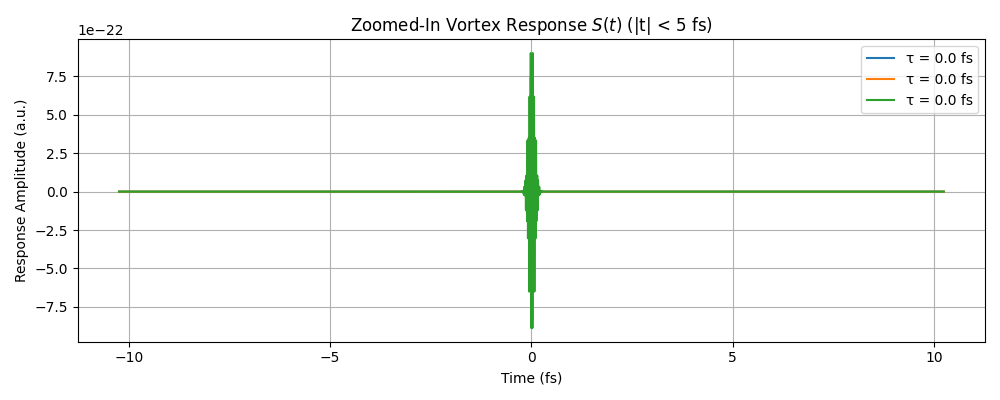
\includegraphics[width=0.75\textwidth]{images/vam_time_response_zoom_plot}
  \caption{Zoomed view of $S(t)$ around $t = 0$, highlighting the coherent coupling for longer pulses. The narrow-band excitation leads to smoother and more resonant vortex activation.}
\end{figure}

\end{document}
